\documentclass[12pt,a4paper,twocolumn]{article}
% The following LaTeX packages must be installed on your machine: amsmath, authblk, bm, booktabs, caption, dcolumn, fancyhdr, geometry, graphicx, hyperref, latexsym, natbib
\input{151.dat}
\usepackage{gensymb}
\usepackage{float}
\usepackage{siunitx}
\usepackage{amssymb}
\usepackage{float}
\usepackage{enumerate}
\usepackage{listings}
\PassOptionsToPackage{hyphens}{url}\usepackage{hyperref}
\usepackage[none]{hyphenat}
%\renewcommand{\familydefault}{\sfdefault}


\begin{document}

\setcounter{page}{1}

\section*{Problem 1.8}
\begin{enumerate}[(a)]

\item Using parameters $N = 40$, $E = 40$, and $d = 3$, the mean energy of the demon $\langle E_d \rangle$, after running the program for some time, starts to approach a steady value.

\item After running the program for a reasonable time ($> 100000$ mcs), the mean energy of the demon $\langle E_d \rangle$ appears to have stabilized at a value of 0.655, while system mean energy $\langle E \rangle$ appears to have stabilized at a value of 39.345, which corresponds to a $\langle E \rangle / N$ value of 0.984, indicating that the mean energy per particle is greater than the demon's mean energy. The ratio $\nu = \frac{\langle E_d \rangle}{\langle E \rangle / N}$ is 0.667.

\item Doubling the value of $E$ and running the program for the same amount of time, $\langle E_d \rangle$ and $\langle E \rangle / N$ respectively approach values of 1.308 and 1.967, corresponding to the ratio $\nu = 0.665$.

\begin{table}[ph!]
    \centering
    \caption{Energy values for different $N$ and $E$.}
    \label{tab:energy}
    \begin{tabular}{|c|c|c|c|c|c|}
        \hline
        $N$ & $E$ & $\langle E_d \rangle$ & $\langle E \rangle$ & $\langle E \rangle/N$ & $\nu$ \\ \hline \hline
        40 & 40 & 0.655 & 39.345 & 0.984 & 0.667 \\ \hline
        60 & 40 & 0.436 & 39.564 & 0.659 & 0.662 \\ \hline
        80 & 40 & 0.331 & 39.669 & 0.496 & 0.667 \\ \hline
        100 & 40 & 0.265 & 39.735 & 0.397 & 0.667 \\ \hline
        40 & 80 & 1.308 & 78.692 & 1.967 & 0.665 \\ \hline
        60 & 80 & 0.879 & 79.121 & 1.319 & 0.667 \\ \hline
        80 & 80 & 0.66 & 79.34 & 0.992 & 0.665 \\ \hline
        100 & 80 & 0.532 & 79.468 & 0.795 & 0.669 \\ \hline
    \end{tabular}
\end{table}

\begin{figure}[htb]
	\centering
	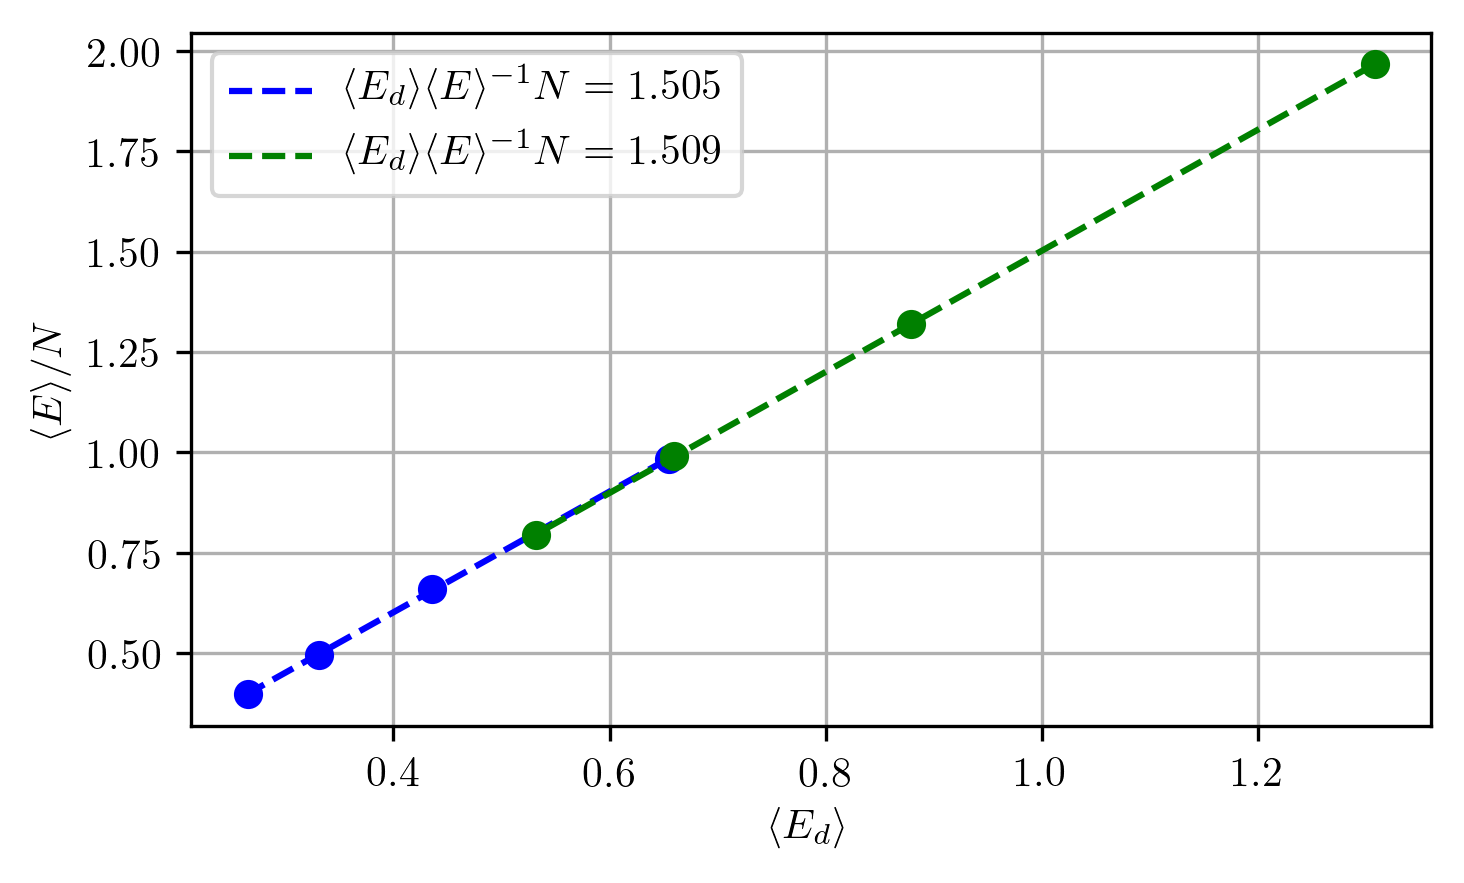
\includegraphics[width=0.45\textwidth]{demonenergy.png}
	\caption{Plot showing the relation of the mean demon energy and mean system energy.}
	\label{fig:energy}
\end{figure}

By varying the values of $N$ and $E$, a linear relation between the mean demon energy and mean system energy can be observed, as shown in Table \ref{tab:energy} and Figure \ref{fig:energy}. The ratio $\nu$ remains fairly constant, and via linear regression, this value appears to be in the neighborhood of $1.507 \approx 3/2$, which corresponds to a familiar relation

\begin{equation}\label{eq:famrelation}
	\frac{\langle E \rangle}{N} = \frac{3}{2} \langle E_d \rangle.
\end{equation}

\item From the mean energy of an ideal gas in 3 dimensions and rearranging some terms,

\begin{equation}\label{eq:idealgas}
	\frac{\langle E \rangle_{ideal}}{N} = \frac{3}{2} k_B T
\end{equation}

Comparing this with \eqref{eq:famrelation}, it is evident that

\begin{equation}\label{eq:parallel}
	k_B T \propto \langle E_d \rangle
\end{equation}

but then, we have set units of $k_B = 1$. Therefore,

\begin{equation}
	T \propto \langle E_d \rangle
\end{equation}


\item 

\end{enumerate}

\end{document}